% !TEX TS-program = LuaLaTeX
\documentclass[10pt, oneside, a4paper]{article}

\usepackage[T1]{fontenc}
\usepackage{lmodern}
\usepackage{xcolor}
    \definecolor{gray} {HTML}{363636}
    \definecolor{red}  {HTML}{950009}
    \definecolor{green}{HTML}{0E610A}
    \definecolor{blue} {HTML}{020069}
\usepackage{fontspec}
    \setsansfont{Arial}
\usepackage{amsmath}
\usepackage{titlesec}
    \titleformat*{\section}      {\color{gray}\large\bfseries\sffamily}
    \titleformat*{\subsection}   {\color{gray}\large\bfseries\sffamily}
    \titleformat*{\subsubsection}{\color{gray}\large\bfseries\sffamily}
\usepackage{geometry}
%   \geometry{showframe}
    \geometry{scale={0.75,0.85}}
%\usepackage{pgfplots}
%    \pgfplotsset{compat=newest}
\usepackage{siunitx}
    \sisetup{locale=FR}
\usepackage{graphicx}
\usepackage{caption}
    \captionsetup{labelfont={bf,sf,color=gray}}
\usepackage{pdfpages}

% Keep lasts
\usepackage[french]{babel}
	\frenchsetup{SmallCapsFigTabCaptions=false}
\usepackage[expansion]{microtype}
\usepackage[luatex, backref]{hyperref}
    \hypersetup{unicode, colorlinks, breaklinks, urlcolor=red,
                bookmarksopen, bookmarksnumbered}

\renewcommand{\UrlFont}{\small}
\renewcommand{\arraystretch}{1.1}
\newcommand{\important}[1]{\textbf{\textsf{\color{gray}{#1}}}}
\setlength{\parskip}{2mm}

\begin{titlepage}
    \date{%
        \today
    }
    \author{%
        Alexis~\bsc{Nootens} \\
        \href{mailto:16139@student.ecam.be}{16139@student.ecam.be}
        \and
        Thomas~\bsc{Anizet} \\
        \href{mailto:14164@student.ecam.be}{14164@student.ecam.be}
    }
    \title{%
        \color{gray}\LARGE\bfseries\sffamily
        Rapport de bureau d'étude                  \\[3mm]
        \rm\sffamily\large
        Réalisation d'un amplificateur de classe D \\[7mm]
        École Centrale des Arts et Métiers 		   \\
        1200 Woluwe-Saint-Lambert				   \\
        Belgique
    }
\end{titlepage}

\begin{document}
\maketitle

%%%%%%%%%%%%%%%%%%%%%%%
\section*{Introduction}
	\pdfbookmark[1]{Introduction}{sec:intro}
Après avoir étudié la théorie derrière le transfert de puissance en électronique,
nous avons mis à l'épreuve nos acquis théoriques dans un cas pratique en réalisant un circuit d'amplification de signaux audio analogiques.
Ce circuit d'amplification appartient à la classe D, une classe exploitant la connaissance de l'électronique de puissance, pour minimiser les pertes d'énergies aux étages d'amplification.
Ce document reprend notre réalisation et notre analyse du circuit.


%%%%%%%%%%%%%%%%%%%%%%%%%%%%%%%%
\section{Hypothèses considérées}
Avant de s'attaquer au problème, définissons l'environnement dans lequel nous allons travailler tel que la nature du signal reçu en entré.
Notre amplificateur doit être conçu pour les signaux audio ;
les signaux audio sont produit par un module convertisseur analogique-numérique (sigle CAN, ou DAC en anglais).
Leur tension est asymétrique entre \num{0} et une référence observée habituellement à \SI{2048}{\milli\volt} et leur fréquence varie entre \num{20} et \SI{22000}{\hertz}~\cite{heffner2007hearing}.
Nous supprimerons donc les composantes fréquentielles hors de ces bornes par des filtres passe-haut et passe-bas.


%%%%%%%%%%%%%%%%%%%%%%%%%%%%%
\section{Principes exploités}
Le circuit réalisé repose sur deux modules pour amplifier le signal d'entré :
un convertisseur analogique-numérique de type Sigma-Delta, et un contrôleur de transistor MOSFET.
La mise en série de ces deux modules permet de créer un amplificateur de classe D.
Les sous-sections \ref{sec:sigmaDelta} et \ref{sec:classeD} définissent le principe derrière chaque module et évoquent leur raison d'être.


\subsection{Modulation Sigma-Delta}
	\label{sec:sigmaDelta}
Il existe une évolution des méthodes de modulation en pleine onde.
La plus simple est la modulation de largeur d'impulsion, MLI.
% Modulation de Largeur d'Impulsion
Voici comment elle fonctionne : depuis deux états possibles de tension, haut et bas, une période d'impulsion nommée \tau, et une durée variable de tension haute nommée $t$, le signal respecte la condition suivante : $0 \leq t \leq \tau $, soit $t \div \tau \in [0,1]$.
L'information modulée se situe dans le rapport de durée tension haute sur durée d'impulsion.
La donnée nécessite d'être transposée au préalable dans l'interval entre 0 et 1.
Cette modulation bénéficie de pouvoir être directement applicable comme commande d'un étage d'amplification en puissance.
Elle se traduit sans opération supplémentaire en commande complètement ouverte ou complètement fermée de transistor.

% Modulation Delta
Une évolution de la modulation de largeur d'impulsion est la modulation Delta.
Tandis que la MLI encode l'entièreté de l'information dans son rapport cyclique à chaque période, la modulation Delta n'encode que la différence (delta) par rapport à l'information précédente.
Les différences entre informations sont de taille plus petites que les informations entières.
Elles sont envoyées plus rapidement.
Ainsi, pour une période donnée, plus de delta pourront être envoyés que de cycles MLI complets.
Le modulateur fonctionnera à une fréquence plus élevée, suréchantillonnant le signal, ce qui réduit le bruit de quantification~\cite{gray1998quantization} par rapport à un modulateur MLI.

% Modulation Sigma-Delta
La modulation Delta connecte la sortie à l'entrée pour la différentier, c'est une rétro-action.
Un automaticien y reconnaîtra un contrôle en boucle fermée proportionnel, un régulateur P.
Cet automaticien saura également que ces régulateurs ont le défaut de toujours avoir un décalage entre la consigne et le signal de sortie désiré, nommé \og écart statique \fg{}.
Ce problème se résout en ajoutant un intégrateur avant la comparaison ; ce dernier maintient la dernière valeur comparu.
Cela devient un régulateur PI \og proportional-integral \fg{}.
Cette nouvelle modulation se nomme \important{Sigma-Delta}, puisqu'elle somme (\Sigma) les différences (\Delta).

Le schéma fonctionnel d'un circuit sigma-delta est présenté à la figure~\ref{fig:sigmaDelta}.
Voici son fonctionnement :
pour un signal d'entrée constant non nul, le différentiateur débute par soustraire le signal de sortie à l'entrée.
Si le système est reposé, la sortie est nulle et le signal d'entrée arrive pleinement à l'intégrateur.
L'intégrateur va introduire une temporisation dans le système ;
le signal à la sortie de l'intégrateur grimpe progressivement de manière monotone.
Ce signal arrive à l'entrée d'un comparateur qui retourne une tension soit maximale, soit minimale.
C'est ce signal binaire qui est réutilisé en rétro-action.
Le système va tenter de compenser le signal d'entrée avec la tension haute ou la tension basse.
Cette tension n'ayant pas de valeur intermédiaire, le système ne parviendra jamais à compenser le signal d'entré si celui-ci se trouve entre les bornes.
Le système est oscillant.
L'information modulée s'encode comme les différences entre cycle tension haute -- basse.

\begin{figure}[tbp]
    \centering
    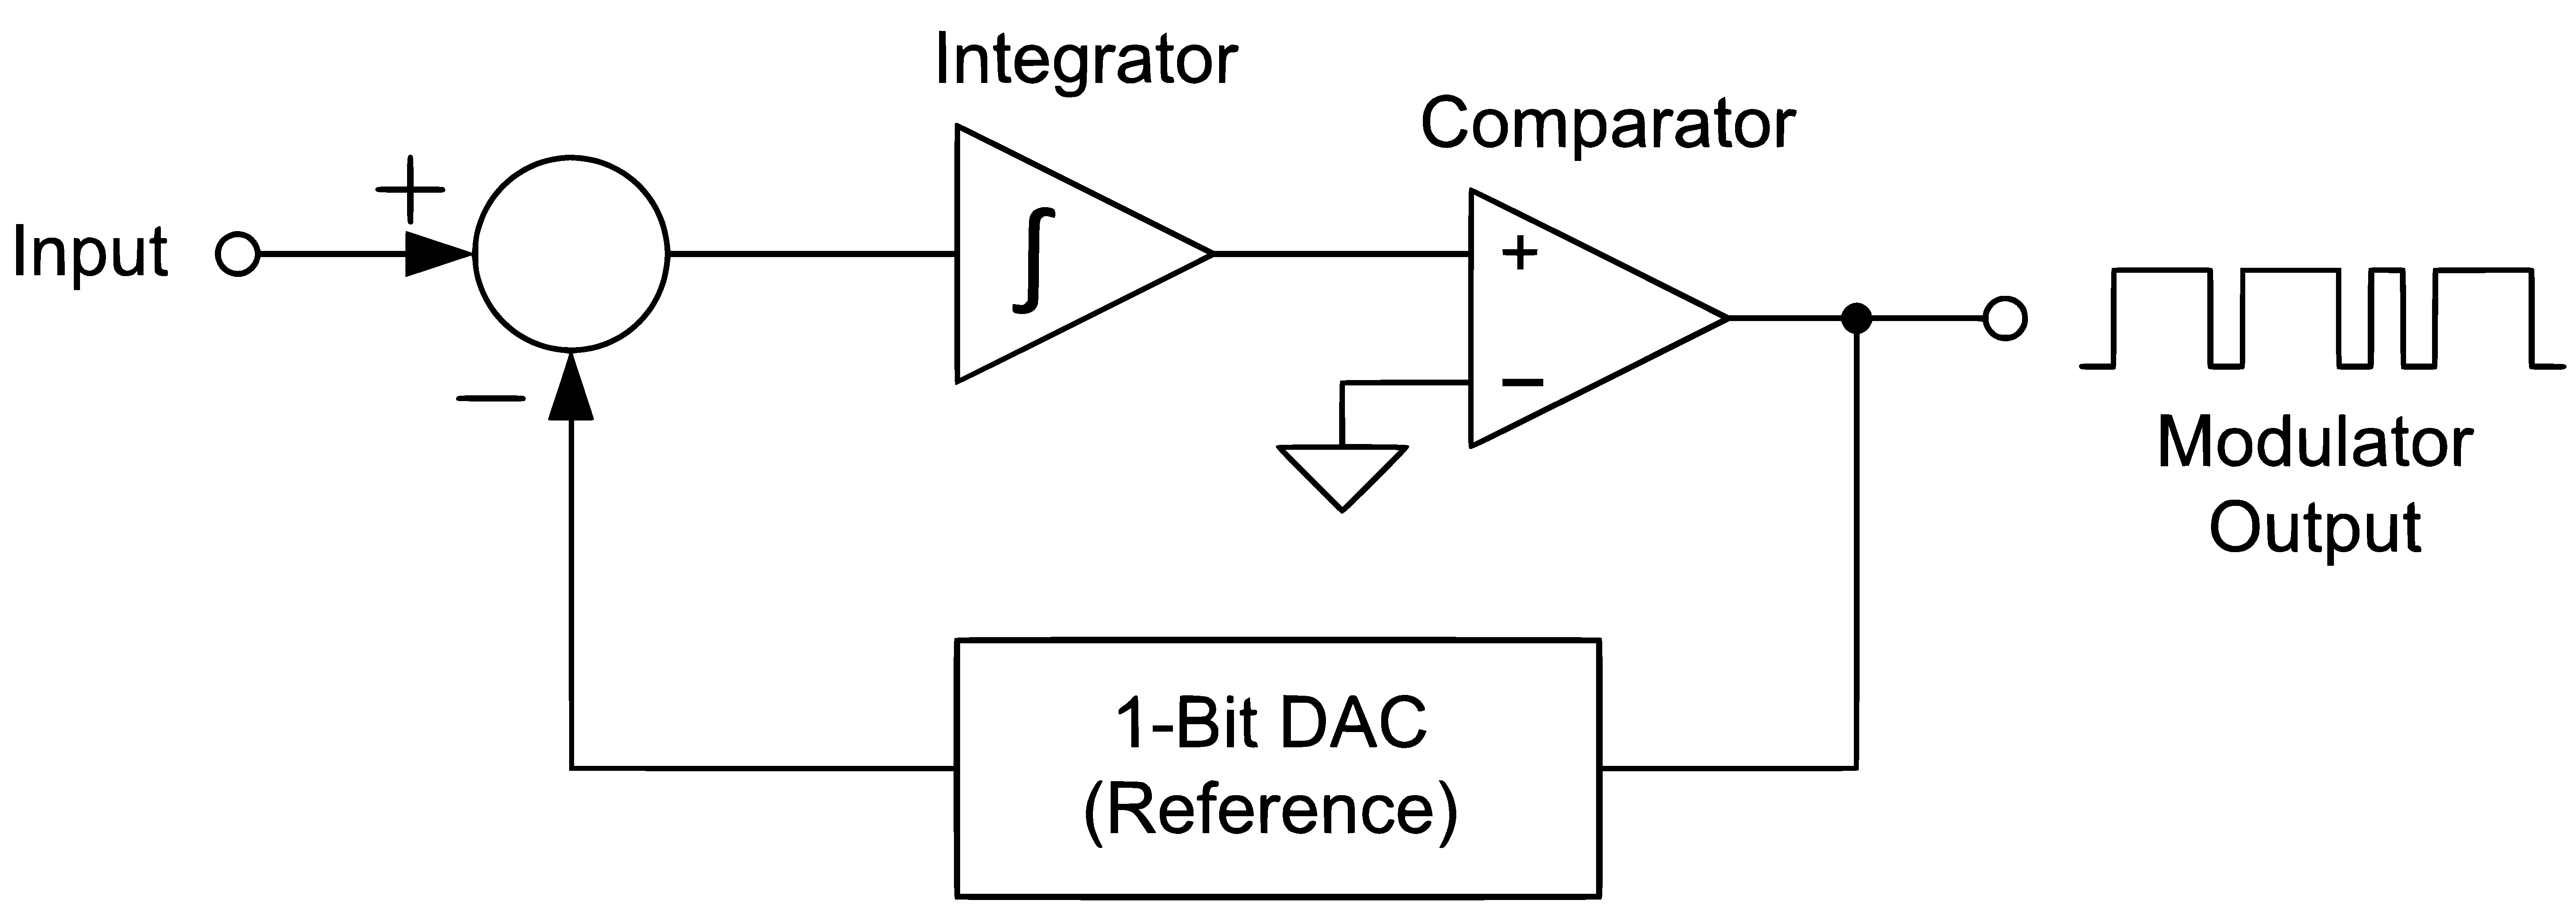
\includegraphics[width=0.7\textwidth]{eps/sigma-delta.eps}
    \caption{Schématique symbolique d'un modulateur \Sigma-\Delta.
    Le signal d'entrée \og Input \fg{}{} est de nature analogique.
    Le circuit agit en boucle fermée pour compenser la différence entre entrée et sortie.}
    \label{fig:sigmaDelta}
\end{figure}


\subsection{Amplificateur de classe D}
	\label{sec:classeD}
La famille des amplificateurs contient plusieurs division --- dénommées \og classes \fg{} --- selon la nature du signal en sortie.
Par exemples :
les amplificateurs de classe A sortent une tension sinusoïdale amplifiée sur les deux crêtes ;
les amplificateurs de classe B ne laissent sortir qu'une seule crête amplifiée du sinus.

Les amplificateurs de classe D imposent des tensions aux rails d'alimentation du circuit.
C'est du tout ou rien.
Ils sont composés de transistor MOSFET.
Les transistors MOSFET sont les favoris de l'électronique de basse puissance.
Ils peuvent travailler à haute fréquence (plusieurs dizaines de kHz) et leur résistance à la conduction en saturation \og $\text{R}_{\text{DS,ON}}$ \fg{} est très faible (une centaine de m\Omega{} dans les basses puissances)~\cite{irf2017mosfet}.
Cette propriété donne tout son intérêt au amplificateur de classe D.
En ouvrant ou fermant complètement les transistors pour les faire fonctionner dans leur zone saturée, on minimise la résistance de conduction.
Sachant que la perte en conduction est dû à l'effet joule, et que la puissance de l'effet joule se formule comme $P=RI^2$~\cite{griffiths1999introduction}.
Lorsque $R$, la résistance du transistor est minimale, la puissance $P$ perdue à la conduction est minimisée pour une courant $I$ donné~\cite{sente2017elec}.
Le principe de l'amplificateur de classe D est présenté visuellement à la figure~\ref{fig:classeD}.
Un filtre LC peut-être placé à la suite de l'étage d'amplification pour lisser le courant et la tension~\cite{wildi2005electrotech}.
Dans notre réalisation, nous considérons que le bobinage du haut-parleur lissera le courant et nous ne placerons pas d'inductance discrète.

\begin{figure}[tbp]
    \centering
    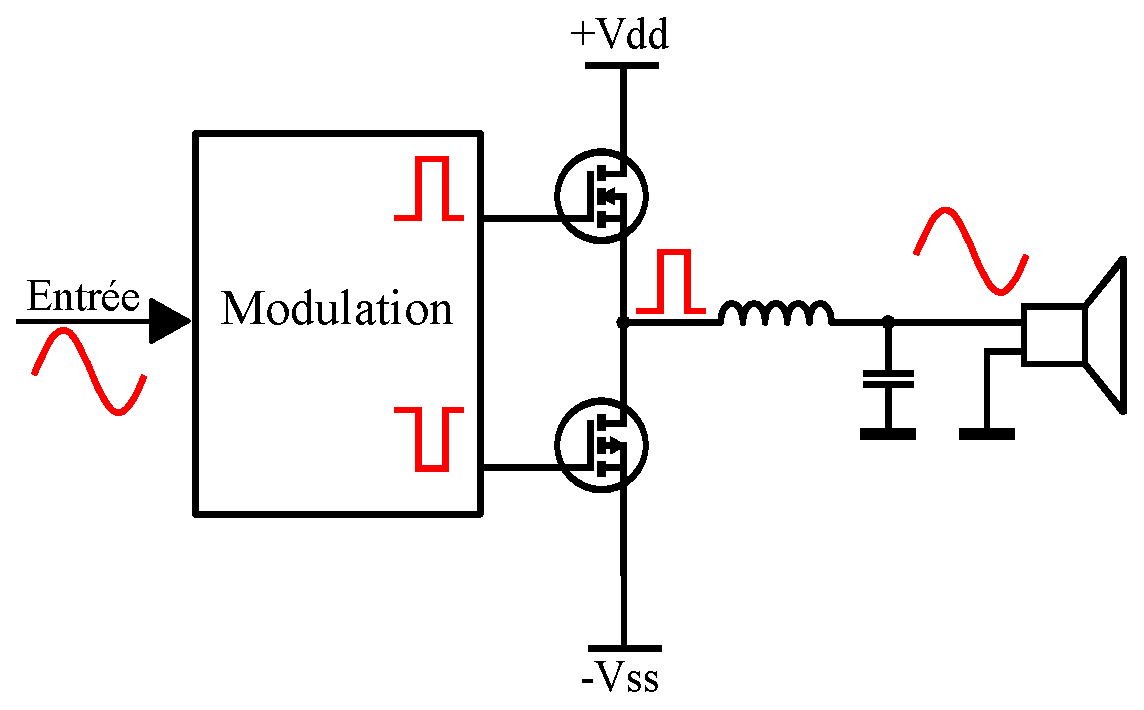
\includegraphics[width=0.5\textwidth]{eps/classe-d.eps}
    \caption{Schématique du principe de l'amplificateur de classe D.
    Le signal d'entré analogique est modulé en commande de commutation de transistor de puissance.
    Le signal amplifié se trouve à l'état $+\text{Vdd}$ ou $-\text{Vss}$ uniquement.
    Ce signal est ensuite lissé au travers d'un filtre LC pour retrouver des tensions intermédiaires.}
    \label{fig:classeD}
\end{figure}


%%%%%%%%%%%%%%%%%%%%%%%%%%%%%%
\section{Schématique du circuit}


%%%%%%%%%%%%%%%%%%%%%%%%%
\section{Dimensionnement}

\subsection{Filtre pré-amplification}
\subsection{Filtre RC}
\subsection{Constante de temps du Sigma-Delta}


%%%%%%%%%%%%%%%%%%%%%%%%%%%%
\section{Analyse du circuit}
Après que les éléments aient été dimensionnée, nous avons opté pour analyser le circuit en le faisant fonctionner en régime normal et en prenant des mesures en différents points.
Ces mesures sont toujours, sauf si cité explicitement, en tension par rapport à la masse, elle même mise à la terre.

\subsection{Défaut de fabrication}
Dés le premier branchement de la carte en tension symétrique \pm\SI{25}{\volt}DC,
nous avons observé un appel de courant de \SI{200}{\milli\ampere} sur le circuit.
Cette valeur était le maximum paramétré sur l'alimentation de laboratoire à notre portée.
Ce courant est trop élevé pour un amplificateur au repos, c.-à-d. sans signal d'entrée.
Il n'y a nul doute qu'un problème de connexion existe sur la carte.

Pour cerner le problème, nous avons connecté un ohmmètre entre les bornes d'alimentation : positive-négative, positive-neutre, neutre-négative.
À ces bornes nous avons mesuré respectivement une résistance de : \SI{33}{\Omega}, \SI{9}{\kilo\Omega} et \SI{9}{\kilo\Omega}.
C'est désormais déterminé et mesuré, il existe un défaut de connexion entre la borne positive et le neutre.

Une analyse bloc-par-bloc a permis de déterminer que le problème était le circuit intégré \verb|TC4428|, un double inverseur présentant un courant de fuite de \SI{100}{\milli\ampere} pour une tension d'alimentation de seulement \SI{4.3}{\volt};
ce qui est déraisonnable et en opposition avec la fiche technique du produit.
Nous en avons déduit que le composant était détruit.

Après avoir remplacé le circuit intégré \verb|TC4428|, nous avons observé que la résistance entre la borne d'alimentation positive et le neutre passait de \SI{33}{\Omega} à \SI{200}{\Omega}, ce qui n'est toujours pas acceptable.
Nous avons remplacé un second circuit intégré douteux, le \verb|L6385E|, et la résistance est passée de \SI{200}{\Omega} à \SI{19}{\kilo\Omega}; ce qui est désormais raisonnable.
Tout cela démontre que deux des circuits imprimés ont été détruits.
Nous ne savons pas déterminer l'instant auquel cela s'est produit.


%%%%%%%%%%%%%%%%%%%%%
\section*{Conclusion}
	\pdfbookmark[1]{Conclusion}{sec:conclusion}


%%%%%%%%%%%%%%%%%%
\section*{Crédits}
	\pdfbookmark[1]{Crédits}{sec:credits}
\begin{itemize}

\item Figure~\ref{fig:sigmaDelta} provenant de :\\*
Le blog officiel de Texas Instrument :
\url{https://e2e.ti.com/blogs_/archives/b/precisionhub/archive/2015/01/21/delta-sigma-adc-basics-understanding-the-delta-sigma-modulator}

\item Figure~\ref{fig:classeD} provenant de :\\*
Par Yves-Laurent (Travail personnel) [GFDL (\url{http://www.gnu.org/copyleft/fdl.html}),
CC-BY-SA-3.0 (\url{http://creativecommons.org/licenses/by-sa/3.0/})], via Wikimedia Commons

\end{itemize}

%%%%%%%%%%%%%%%%%%%%%%%%%%%%%%%%%%%%%%%%%%%
\pdfbookmark[1]{Références}{sec:references}
\bibliographystyle{unsrt}
\bibliography{ampli-classe-d}

%%%%%%%%%
\appendix
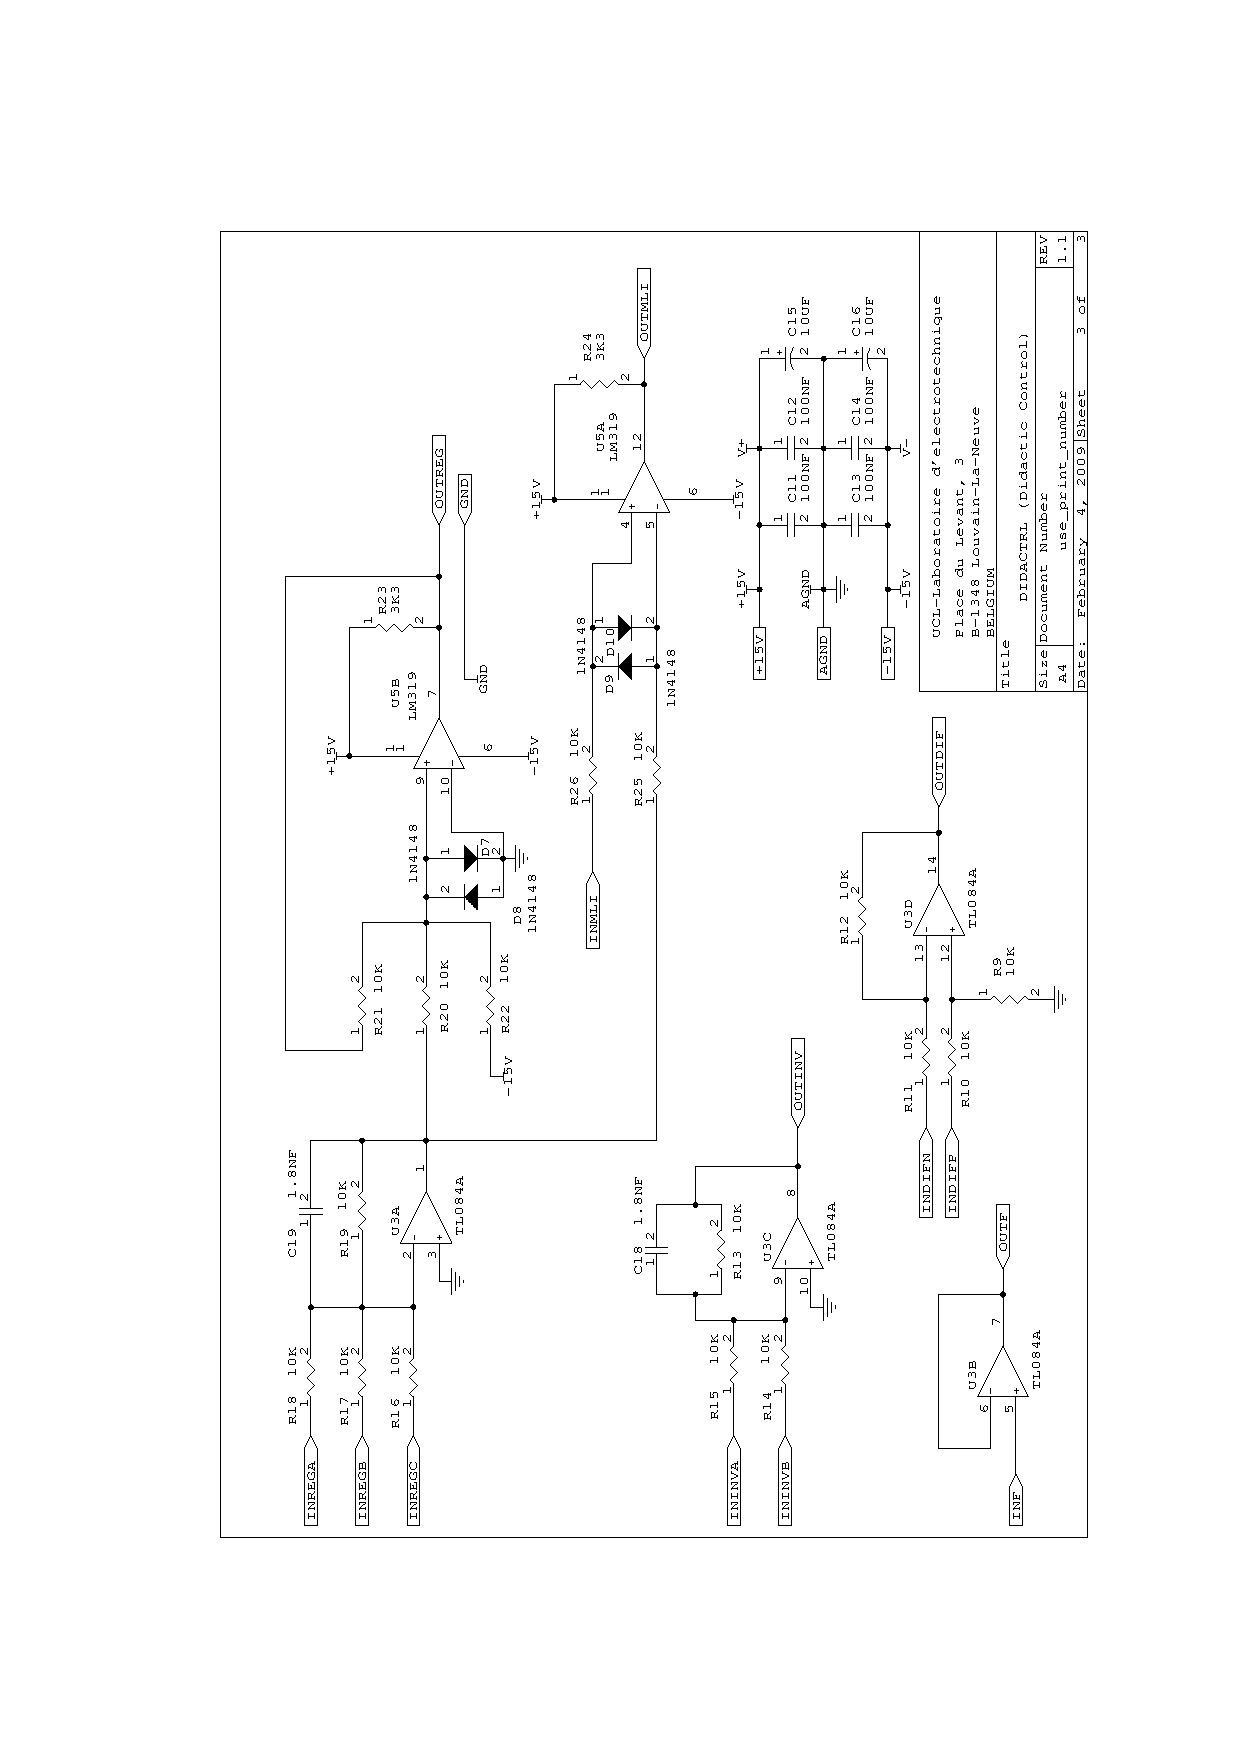
\includepdf[pagecommand=\section{Schéma du circuit DIDACTRL}]{pdf/DIDACTRL.pdf}
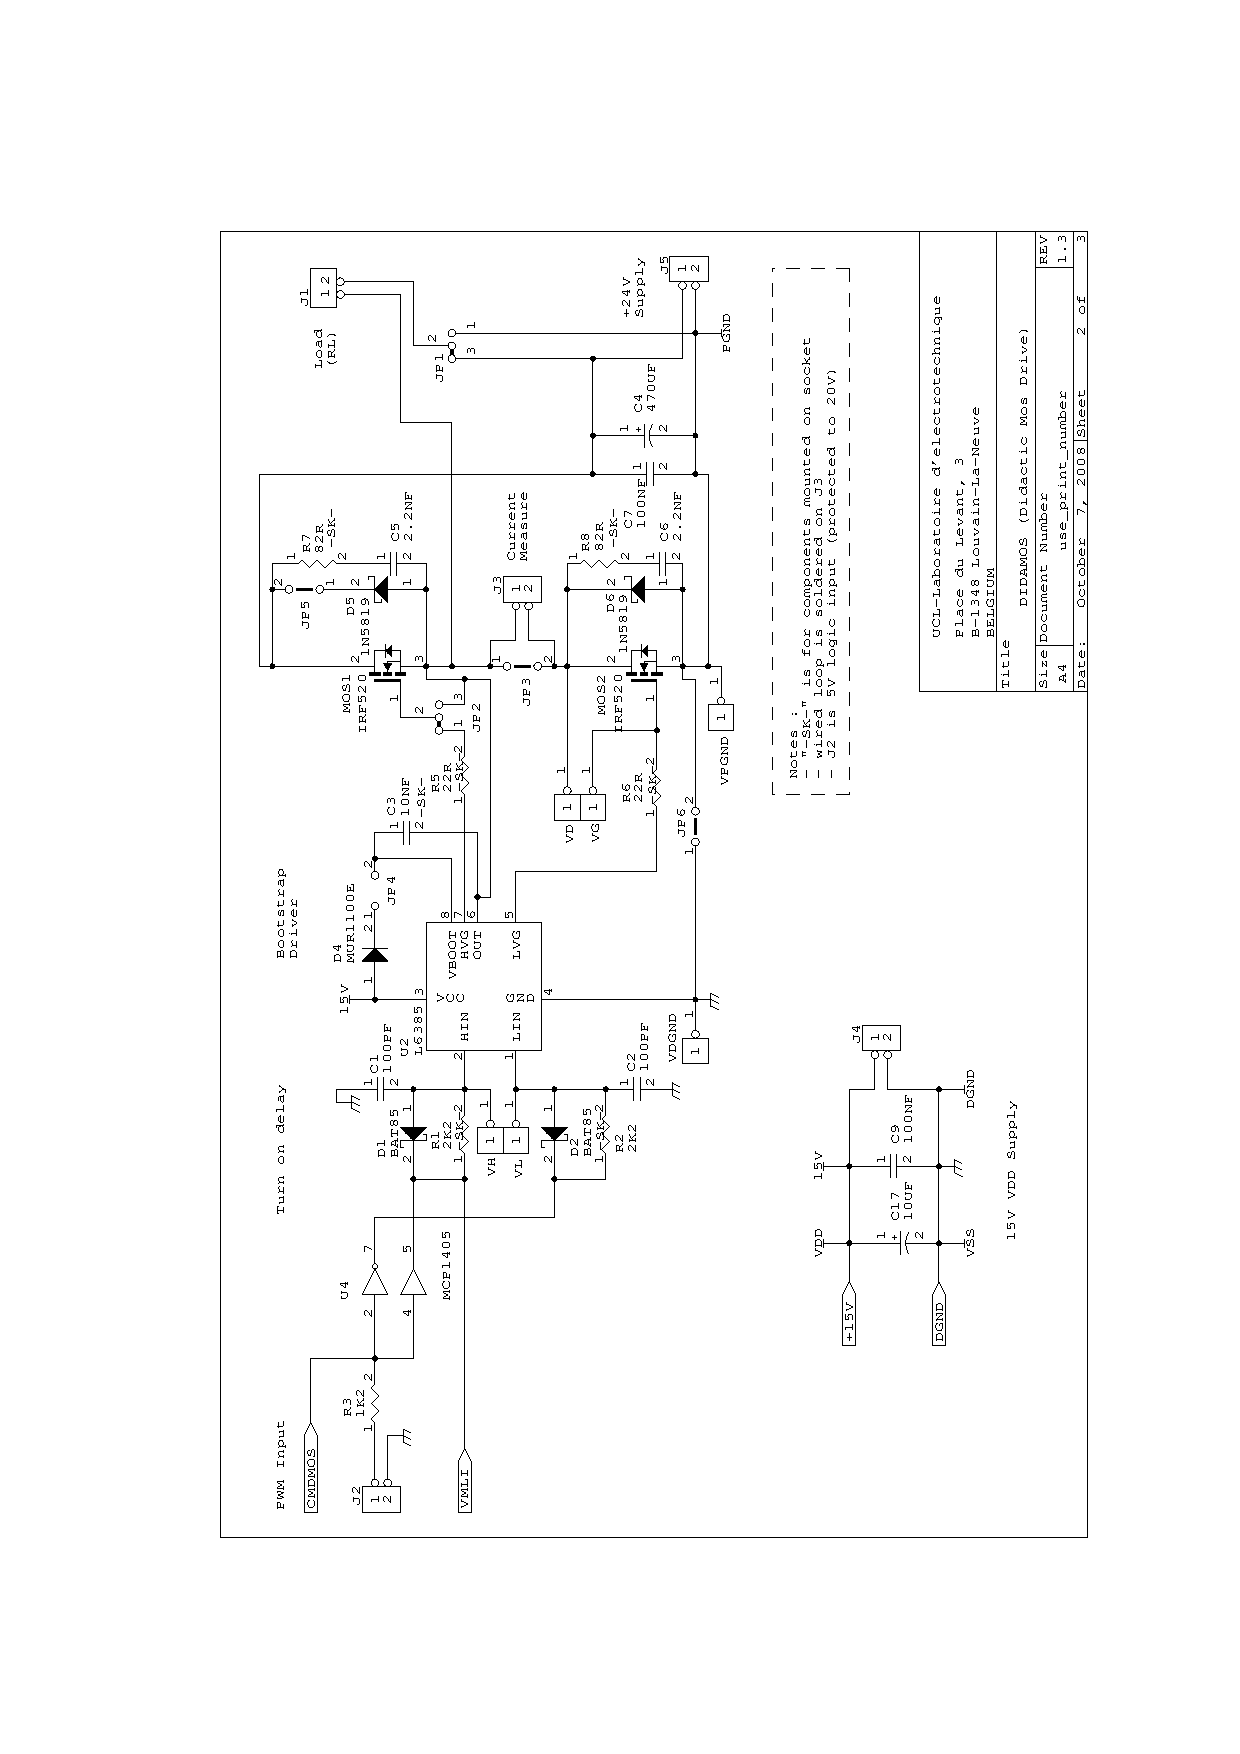
\includepdf[pagecommand=\section{Schéma du circuit DIDAMOS}]{pdf/DIDAMOS.pdf}
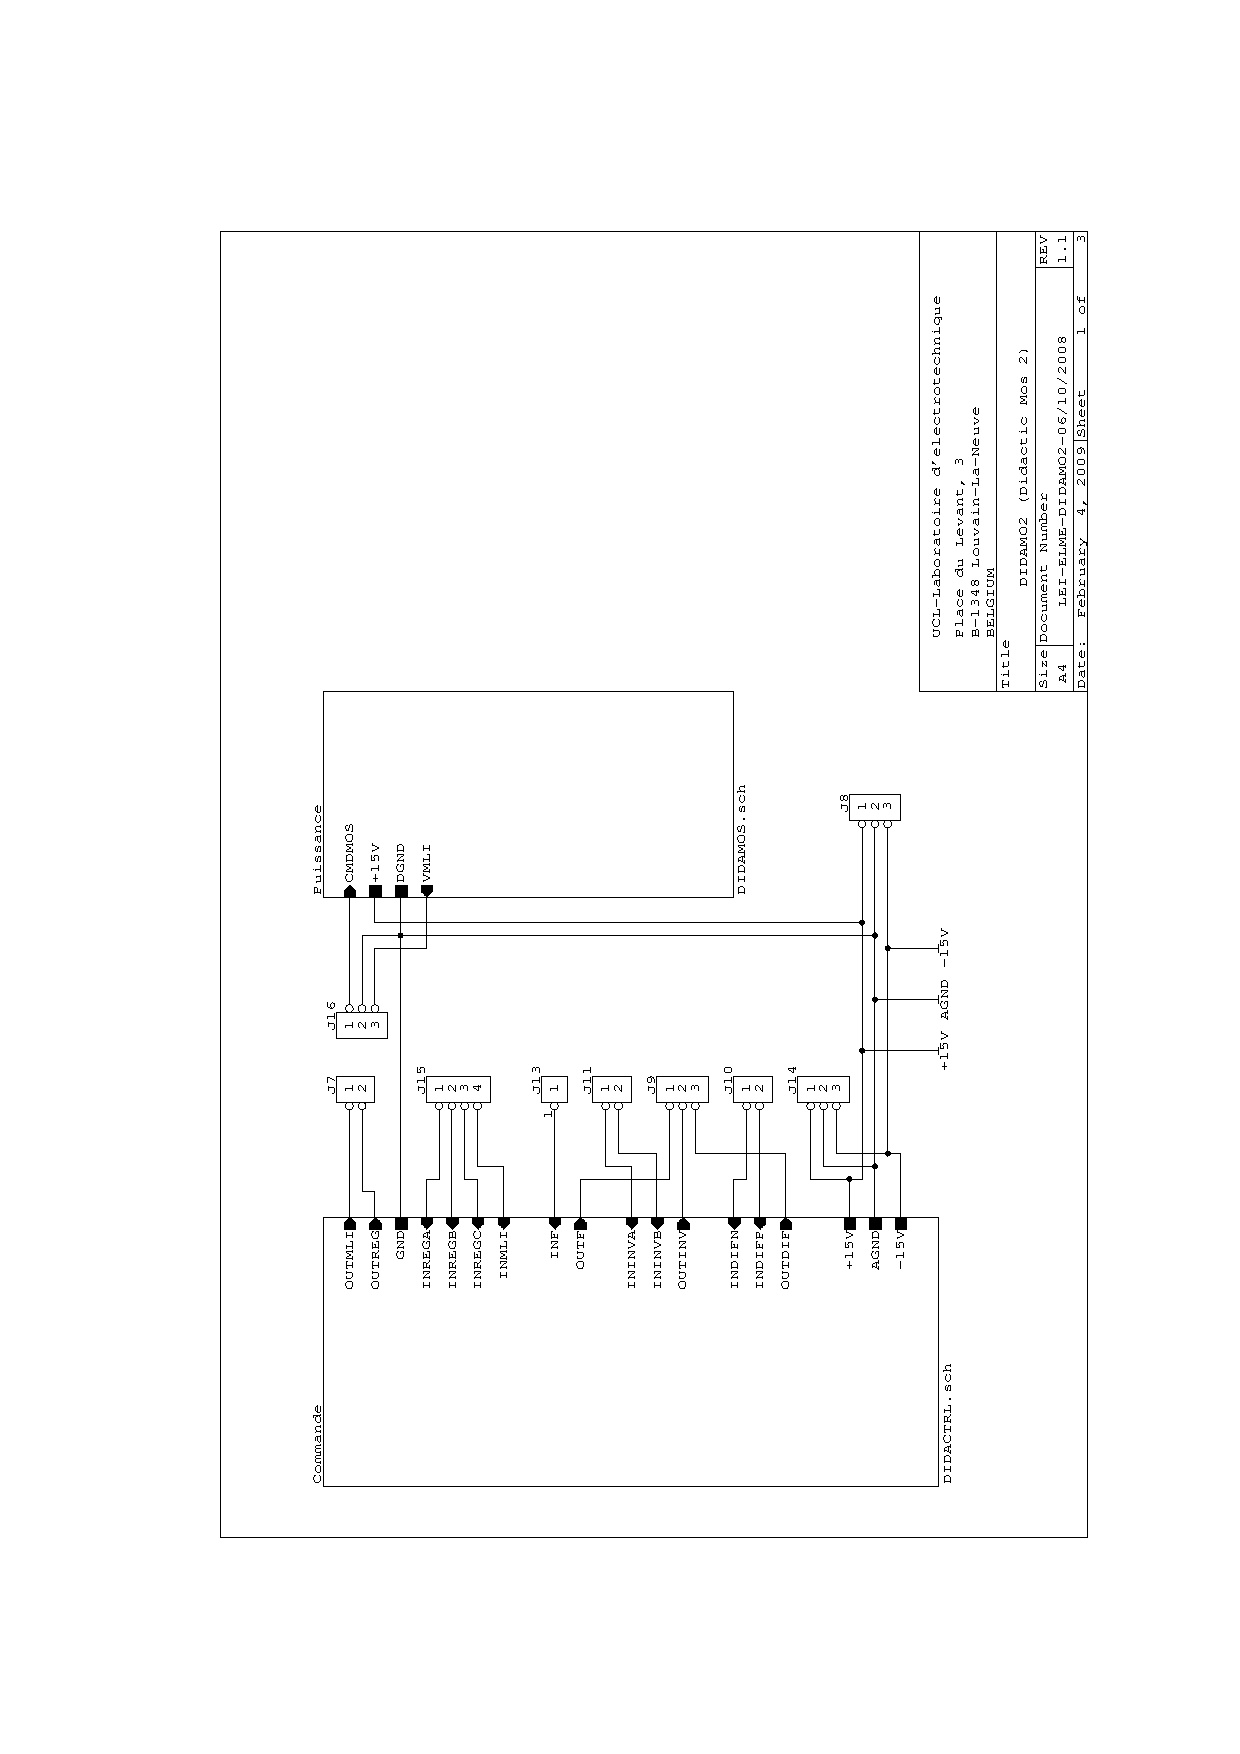
\includepdf[pagecommand=\section{Schéma du circuit DIDAMO2}]{pdf/DIDAMO2.pdf}

\end{document}
